\documentclass[12pt]{article}

\usepackage[english, russian]{babel}
\usepackage[TS1, T2A]{fontenc}
\usepackage[utf8]{inputenc}
\usepackage[left=2cm,right=2cm, top=1cm,bottom=1.5cm,bindingoffset=0cm]{geometry}
\setlength{\parindent}{0cm}
\usepackage{hyperref}
\usepackage{tabularx}
\newcolumntype{b}{X}
\newcolumntype{s}{>{\hsize=.8\hsize}X}
\newcolumntype{m}{>{\hsize=.7\hsize}X}
% \usepackage{multirow}
% \usepackage{hhline}

% \usepackage{indentfirst}

% \usepackage{enumitem,kantlipsum}

\usepackage{graphicx}
\graphicspath{{images/}}

\usepackage{listings}
\lstset{
    language=bash,
    basicstyle=\ttfamily
}
% \DeclareGraphicsExtensions{.pdf,.png,.jpg}

% \usepackage{tikz}
% \usetikzlibrary{patterns}
% \usepackage{pgfplots}
% \pgfplotsset{compat=1.9}
% \usepgfplotslibrary{fillbetween}

% \usepackage{ulem}

% \usepackage{hyperref}

% \usepackage{circuitikz}

% \usepackage{fp}
% \usepackage{xfp}

% \usepackage{siunitx}
% \sisetup{output-decimal-marker={,}}

% \usepackage{minted}

% \let\oldref\ref
% \renewcommand{\ref}[1]{(\oldref{#1})}

\begin{document}
    \pagestyle{empty}
    \begin{center}
        \textbf{Федеральное государственное автономное образовательное учреждение высшего образования}

        \vspace{5pt}

        {\small
        \textbf{САНКТ-ПЕТЕРБУРГСКИЙ НАЦИОНАЛЬНЫЙ ИССЛЕДОВАТЕЛЬСКИЙ УНИВЕРСИТЕТ ИНФОРМАЦИОННЫХ ТЕХНОЛОГИЙ, МЕХАНИКИ И ОПТИКИ}

        \textbf{ФАКУЛЬТЕТ ПРОГРАММНОЙ ИНЖЕНЕРИИ И КОМПЬЮТЕРНОЙ ТЕХНИКИ}%
        }

        \vspace{140pt}

        {\Large
        \textbf{ЛАБОРАТОРНАЯ}

        \vspace{7pt}

        \textbf{РАБОТА №2}%
        }

        \vspace{10pt}

        {\large
        \textbf{Тестирование программного обеспечения}

        \vspace{5pt}

        \textbf{}%
        }

        \vspace{170pt}

        \begin{tabular}{lll}
            Проверил:                                                                                   & \hspace{70pt} & Выполнил:                                             \\
            Сентерев Ю. А.                 \rule[0.66\baselineskip]{1.6cm}{0.4pt}                &               & Студент группы P3455                                  \\
            «\rule[0.66\baselineskip]{1cm}{0.4pt}»  \rule[0.66\baselineskip]{2cm}{0.4pt} \the\year г.   &               & Федюкович С. А. \rule[0.66\baselineskip]{2cm}{0.4pt}  \\
            &               &                                                       \\
            Оценка          \hspace{12pt}           \rule[0.66\baselineskip]{2.7cm}{0.4pt}              &               &                                                       \\
        \end{tabular}

        \vspace*{\fill}

        Санкт-Петербург

        \the\year
    \end{center}
    \newpage
    \pagestyle{plain}
    \setcounter{page}{1}
    \section*{Цель работы}

    Целью данной лабораторной работы является изучение методологий и овладение навыками проектирования тестов.

    В ходе выполнения работы будут получены навыки составления тестовых случаев, а также навыки работы в составе инспекционной группы с подготовкой итогового отчета о выявленных проблемах.

    \section*{Задачи}

    1. Ознакомиться с теоретическими сведениями по методам тестирования.

    2. В соответствии с выбранным заданием(тестовым случаем), подготовить тесты по методикам стратегии "черного ящика"(«белого ящика»).

    3. Тесты свести в таблицу.

    4. Выполнить тестирование. Занести в таблицу результаты

    5. Сделать вывод о роли тестирования с использованием стратегии "черного ящика"(«белого ящика») и возможностях его применения. Сформулировать его достоинства и недостатки.

    \section*{Ход Работы}
    1. С теоретическими сведения ознакомился, готов к выполнению лабораторной работы.

    2. Для тестирования была выбрана программа NPM(Node Package Manager) --- это менеджер пакетов для программной среды Node.js в виде $CLI$. Данная программа написана на языке программирования JavaScript и является очень популярной в среде разработчиков Node.js и имеет открытый исходный код, поэтому для тестирования была выбрана стратегия "белого ящика". Составим тесты и занесём их в таблицу.

    \newpage
    3. Изучив код программы, был составлен следующий список тестов:

    \begin{table}[h]
        \centering
        \begin{tabularx}{\textwidth}{m X s X}
            \hline
            Название теста & Тестовый сценарий & Тестовые данные & Ожидаемый результат \\
            \hline
            Создание модуля с получением ошибок о некорректном названии и версии & В пустой папке запустить создание модуля командой $npm\ init$, ввести в название символы \%, на этапе ввода версии модуля ввести произвольные символы без точек и цифр & нет & Программа выдаёт ошибку о некорректном названии и версии \\
            \hline
            Успешное создание модуля с авто заполнением полей & В пустой папке запустить создание модуля командой $npm\ init$, ничего не вводить на вопросы $npm$, завершить создание модуля & нет & Программа успешно создаёт модуль и $package.json$ файл \\
            \hline
            Установка модуля при некорректном $package.json$ файле & В созданном из предыдущего теста модуле, отредактировать $package.json$ файл, получив некорректный $JSON$, и установить любой модуль при помощи команды $npm\ install$ & Успешно созданный модуль & Программа выдаёт ошибку о невозможности установить модуля по причине неисправности $package.json$ файла \\
            \hline
            Успешная установка модуля & В созданном из прошлого теста модуле установить любой модуль при помощи команды $npm\ install$ & Успешно созданный модуль & Программа успешно устанавливает модуль, добавляя его в $package.json$ \\
            \hline
            Успешное удаление модуля & В созданном из прошлого теста модуле и установленном в нём дополнительном модуле удалить этот установленный модуль при помощи команды $npm\ remove$ & Успешно созданный модуль и установленном к нему дополнительным модулем & Программа успешно удаляет модуль, убирая его из $package.json$ \\
            \hline
        \end{tabularx}
        \caption{План тестирования}
    \end{table}
    \newpage
    4. Для процесса тестирования была создана отдельная папка, в которой и будет происходить запуск тестовой программы. Так же каждый тест подразумевает проверку на то, создавала ли программа лишние файлы или дела ли то, чего не должна.

    В первом тесте запускается создание модуля и вводятся недопустимые символы создание:
    \begin{figure}[h]
        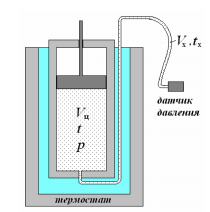
\includegraphics[scale=0.26]{1.png}
        \centering
        \caption{Создание модуля с получением ошибок о некорректном названии и версии}
    \end{figure}

    В следующем тесте запускается создание модуля и не вводятся никакие данные для создания модуля:
    \begin{figure}[h]
        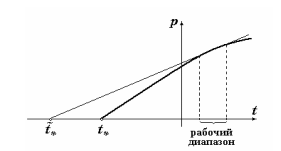
\includegraphics[scale=0.26]{2.png}
        \centering
        \caption{Успешное   создание  модуля с авто заполнением  полей}
    \end{figure}

    \newpage

    В данном тесте проверяется возможность установить дополнительный модуль с неисправным $package.json$ файлом:
    \begin{figure}[h]
        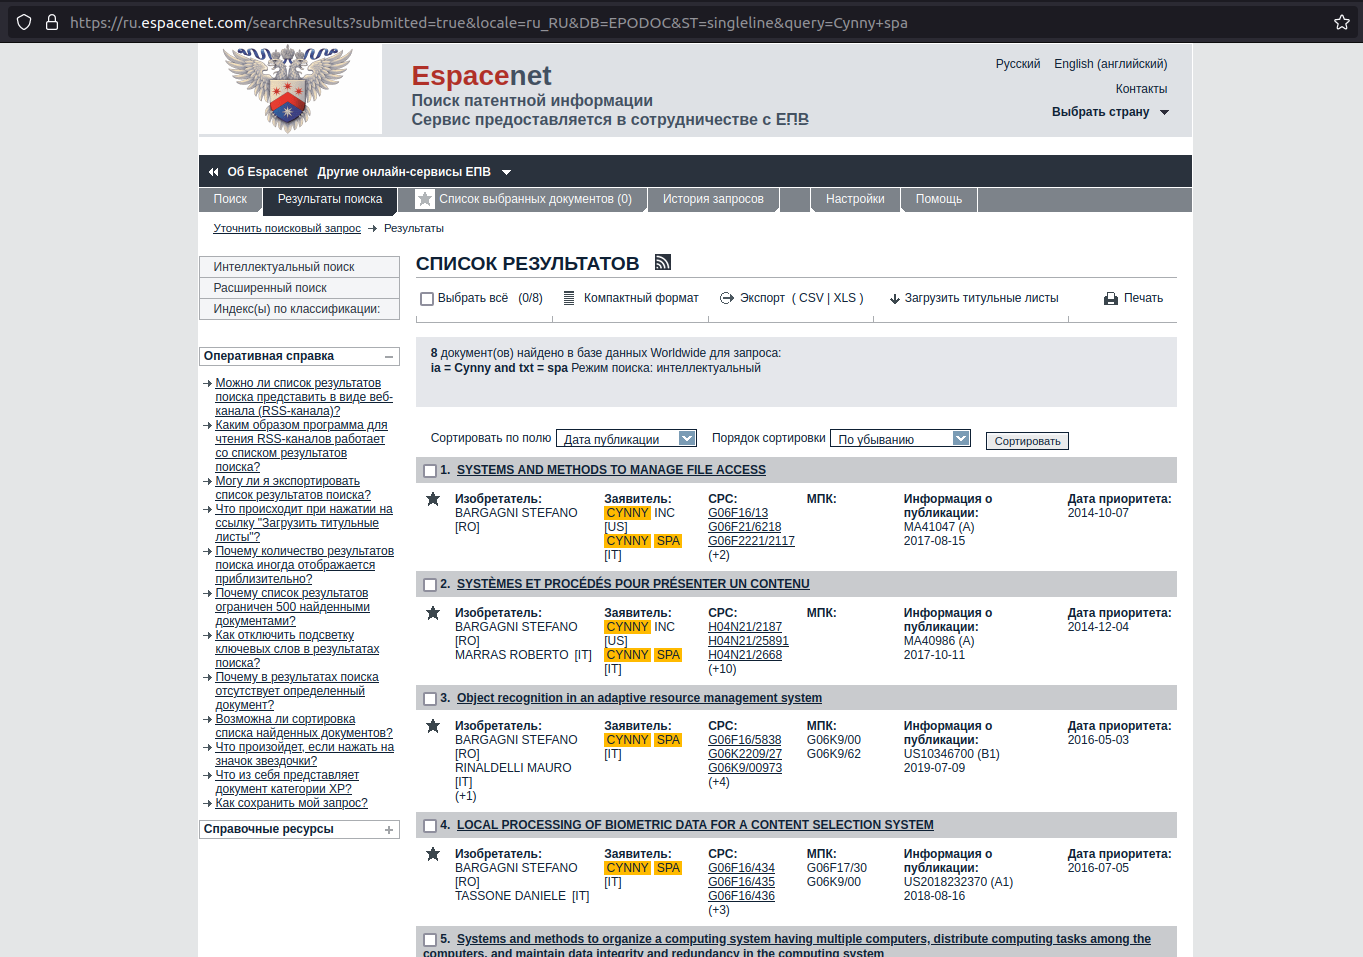
\includegraphics[scale=0.26]{3.png}
        \centering
        \caption{Установка модуля при некорректном $package.json$ файле}
    \end{figure}

    В последующем тесте проверяется возможность успешно установить дополнительный модуль:
    \begin{figure}[h]
        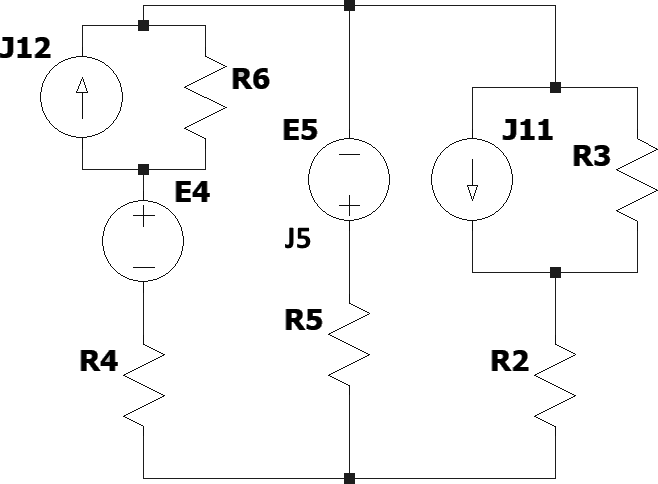
\includegraphics[scale=0.26]{4.png}
        \centering
        \caption{Успешная установка модуля}
    \end{figure}

    \newpage
    В последнем тесте проверяется возможность успешно удалить дополнительный модуль:
    \begin{figure}[h]
        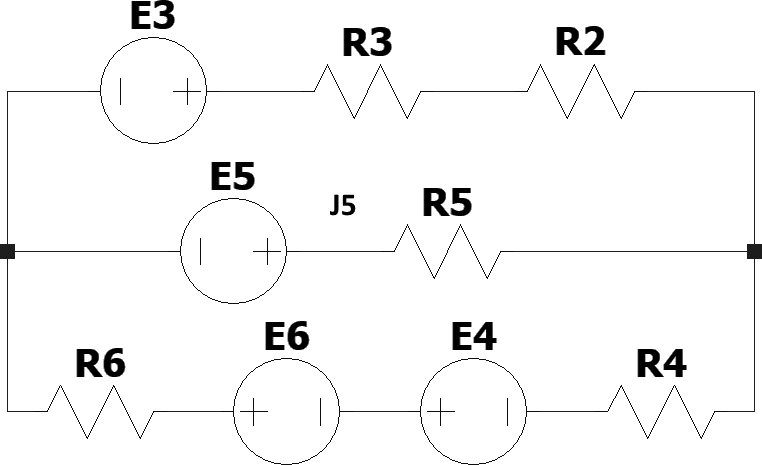
\includegraphics[scale=0.26]{5.png}
        \centering
        \caption{Успешное удаление модуля}
    \end{figure}

    \newpage
    Итоговые результаты тестирования представлены в таблице ниже:

    \begin{table}[h]
        \centering
        \begin{tabularx}{\textwidth}{m X X}
            \hline
            Название теста & Фактический результат & Ожидаемый результат \\
            \hline
            Создание модуля с получением ошибок о некорректном названии и версии & Программа выдаёт ошибку о некорректном названии и версии & Программа выдаёт ошибку о некорректном названии и версии \\
            \hline
            Успешное создание модуля с авто заполнением полей & Программа успешно создаёт модуль и $package.json$ файл & Программа успешно создаёт модуль и $package.json$ файл \\
            \hline
            Установка модуля при некорректном $package.json$ файле & Программа выдаёт ошибку о невозможности установить модуля по причине неисправности $package.json$ файла & Программа выдаёт ошибку о невозможности установить модуля по причине неисправности $package.json$ файла \\
            \hline
            Успешная установка модуля & Программа успешно устанавливает модуль, добавляя его в $package.json$& Программа успешно устанавливает модуль, добавляя его в $package.json$ \\
            \hline
            Успешное удаление модуля & Программа успешно удаляет модуль, убирая его из $package.json$ & Программа успешно удаляет модуль, убирая его из $package.json$ \\
            \hline
        \end{tabularx}
        \caption{Результаты тестирования}
    \end{table}

    Всего было проведено 5 тестов, все из которых были пройдены без ошибок. Процент ошибок равен нулю.

    5. Был сделан вывод о роли тестирования по стратегии белого ящика: тестирование и использование этой стратегии позволяет обнаружить ошибки, специфичные для конкретной реализации программы, которые могли бы быть обнаружены при тестировании стратегией черного ящика. Тестовые сценарии будут меняться только при изменении интерфейса модуля, такие тесты не будут меняться при изменении деталей реализации ПО. С другой стороны, тестирование по стратегии черного ящика может начать разработку тестовых сценариев одновременно с разработкой ПО.

    \section*{Вывод}

    В ходе лабораторной работы я провёл тестирование программы, изучил методологии тестирования ПО и выполнил все поставленные задачи. Лабораторную работу считаю выполненной.

    \section*{Используемая литература}

    1. Гленфорд Майерс, Том Баджетт, Кори Сандлер. Искусство тестирования программ, 3-е издание—М.: «Диалектика», 2015

    2. Бейзер Б. Тестирование чёрного ящика. Технологии функционального тестирования программного обеспечения и систем --- СПб.: Питер, 2004

    3. Канер Кем, Фолк Джек, Нгуен Енг Кек. Тестирование программного обеспечения. Фундаментальные концепции менеджмента бизнес-приложений --- Киев: ДиаСофт, 2001

    4. Винниченко И. Автоматизация процессов тестирования. --- СПб, «Питер», 2018

    5. Котляров В. П., Коликова Т. В. Основы тестирования программного обеспечения --- СПб, Бином. Лаборатория знаний, 2006
\end{document}\